\vspace{-1.5cm}
\small
\textbf{The results in this chapter will be published as:}
\vspace{0.05 cm}

% We cite the paper with fontsize 10
\fullcite{abella2024dynamics}
\normalsize
\vspace{0.5 cm}

This chapter examines the dynamics of real estate housing market from real data from an online listings platforms. By analyzing temporal patterns, we find that market dynamics are non-stationary, with weekly patterns and a steady increase in listings. The data reveals a preferential attachment mechanism, where the likelihood of new listings connecting to an agency depends on the agency's popularity. Additionally, we observe fluctuation scaling in listing prices and distances, highlighting market heterogeneity. The study shows that new listings attach to agencies based on a combination of popularity, price similarity, and spatial specialization. These findings provide insights into the complex interplay of factors driving the housing market, offering a foundation for predicting market trends and improving efficiency.

\section{Introduction}

The use of Internet is widespread in our society and has transformed the way we interact, communicate, and consume information \cite{berners-lee-2006,dorogovtsev2002evolution,pastor-satorras-2004,watts-2007}. New digital platforms have emerged, providing a wide range of services and products, from social media and e-commerce to online banking and food delivery \cite{unknown-author-2013}. The data generated by the human interaction via these digital platforms has become a valuable source of information for researchers, policymakers, and businesses. However, despite the increasing reliance on digital platforms, the extract of reliable knowledge from the data generated by these platforms is still a challenge. The data generated by the human activity in online platforms is often noisy, incomplete, and biased, making it difficult to analyze and interpret. On the other hand, a beter understanding of the way in which users interact in these platforms has important economic consequences, as it can help both the development and monetization of the platforms and the understanding of the interactions between society and these new digital environments \cite{choudary-2016}.

Previous studies on human dynamics using web analytics have demonstrated that, even though human activity in online listings is expected to be unpredictable at an individual level, there are common patterns that emerge at the aggregate level \cite{Lazer2009CompSocSci}. The preferential attachment \cite{barabasi1999emergence,goncalves-2008}, teams self-assembly \cite{guimera-2005}, or the limited social capacity \cite{goncalves-2011,dunbar-2012} are examples of emergent social mechanisms extracted from online platforms data. In this approach, the individual entity is ignored, focussing on the number of interactions, the time between them, or the entities involved in the interactions.

The advent of digital platforms has revolutionized various industries, and the real estate sector is no exception. The increasing reliance on online listings to buy, sell, and rent properties offers a unique opportunity to analyze the underlying dynamics of the housing market through a computational quantitative approach. Online real estate listings provide a rich source of data that can be used to study the temporal and spatial patterns of property transactions, the behavior of real estate agencies, and the preferences of buyers and sellers. With property portals being nowadays the dominant way to create and access market information, online listings constitute a new type of data to study housing markets \cite{sawyer1999ict, boeing2017new, boulay2021moving}. Scholars studied the spatio-temporal distribution of housing prices \cite{yao2018mapping,adolfsen_segmentation_2022}, revealed the persistence of spatial inequalities in the housing information landscape \cite{boeing2020online}, predicted the social profile of neighborhoods \cite{delmelle2021language}, or detected the segmentation of the market from online search patterns \cite{rae2015online}.
Aside price, pictures or textual descriptions, a listing includes a critical piece of information: the identity of the marketing agency that has posted the listing on the portal. As such, listings constitute digital traces \cite{salganikbit2017} of the work performed by real estate agencies when acquiring, selling or marketing on property portals. It is therefore possible to reconstruct, for each agency, its own portfolio of listings, whose volume and location patterns result from and reflect the heterogeneous practices and market shares of real estate agencies. By informing on \textit{who sells where}, listings offer new ways to examine how real estate agencies unevenly operate and specialize across space \cite{palm1976RealEstate}.

\begin{figure}
    \vspace{0.2 cm}
    \centering
    \includegraphics[width =\textwidth]{Figs/Idealista_dynamics/adds_evo.pdf}
	\caption[Active listings evolution.]{\label{fig:active_adds} Daily number of total \textbf{(a)} and active \textbf{(b)} listings during the period 2018 - 2020 for the Barcelona province. The inset in (b) shows a zoomed view to a 1 month period (09-17 to 10-16), where the weekly patterns are more evident.}
\end{figure}

In this chapter, we aim to investigate the dynamics of real estate listings and agencies. Specifically, we seek to answer the following questions: What are the temporal patterns of the listings on the platform? Which is the desicion-making process of a house seller when hiring a real estate agencies ? How the real estate agency prestige, price and location affect this process ? To give an answer to this questions, we examine the real estate agencies dynamics via a temporal bipartite network, where listings are connected to the agency that posted them in a certain temporal window. This methodology is applied to the Spanish market at 3 provinces: Madrid, Barcelona and Balearic islands, using a comprehensive dataset of listings posted on the online platform \texttt{Idealista.com}. For all 3 regions, the dynamics of the market is non-stationary and show non-trivial correlations between the listings metadata in which we are interested: the price, the location and the agency that posted the listing. The results presented in this chapter serve as a basis to understand quantitatively emergent processes such as spatial specialization o price segmentation of the agencies, and could be used to develop models of the housing market dynamics.

\section{Data \label{sec:Data}}

We use the dataset, mentioned in section \ref{sec:Datasets}, of listings published on the online portal \texttt{Idealista.com} \cite{idealista}. The dataset covers a 2-year time period, from January 2017 to December 2018 and it comprises a comprehensive collection of online geolocated listings in the Spanish provinces of Balearic Islands, Barcelona, and Madrid. These listings were posted by real estate agencies for renting or selling residential properties. Posted listings by private individuals are not included into the dataset.

Each listing contains a set of attributes such as the price (in $\textup{\euro}$), the surface area (in $m^2$), the real estate agency that posted it, its location and the dates of both the publication and the removal of the listing. The dataset also contains information about the type of property (e.g. flat, house, etc.), what allowed us to filter rural parcels and commercial properties. We also removed listings with missing or inconsistent information, such as irregular prices or surface areas. Through this chapter, the main results are shown for the selling market, but the same analysis stands for the renting market as well.

\section{Listings dynamics}

\begin{figure}
    \centering
    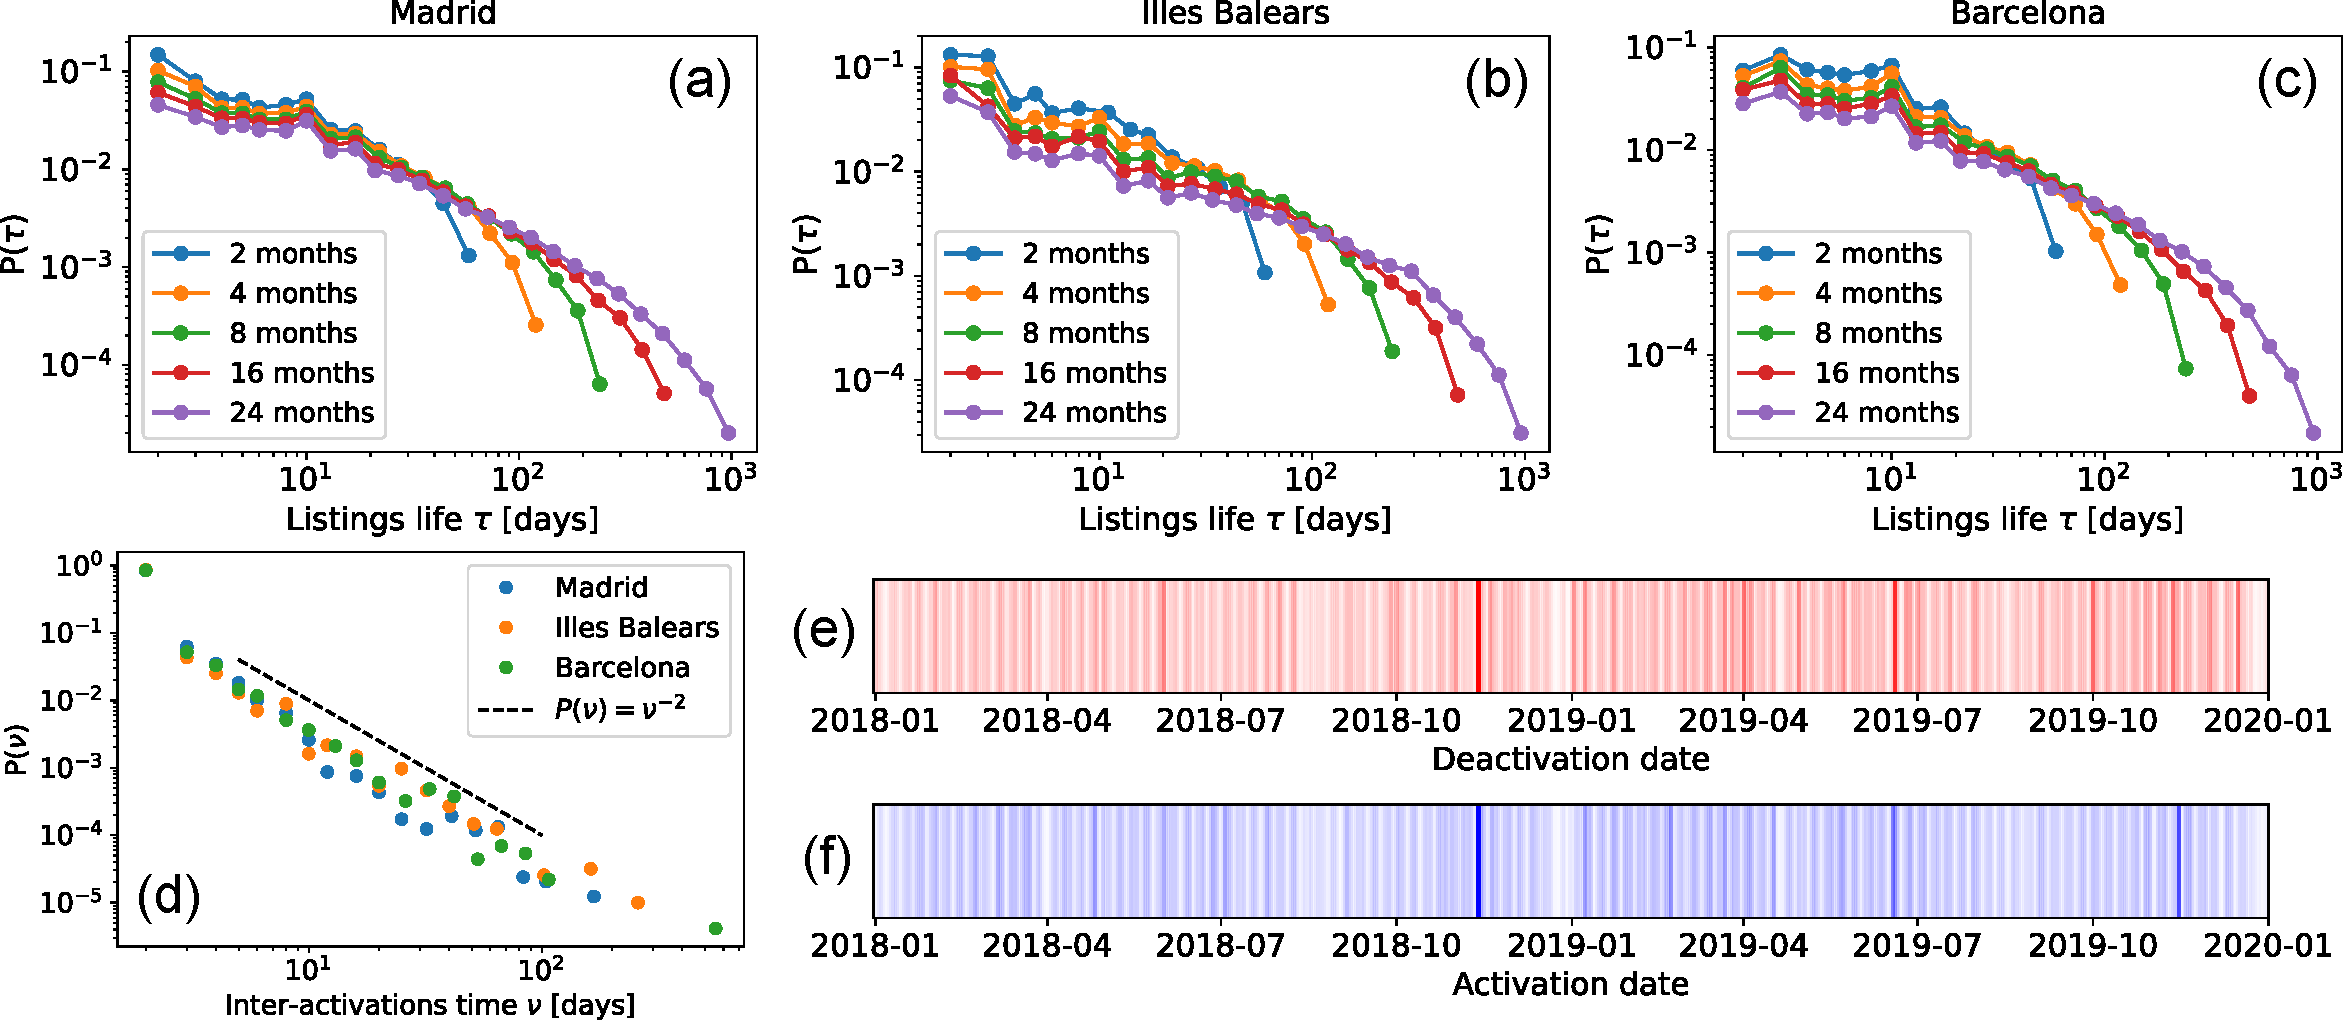
\includegraphics[width =\textwidth]{Figs/Idealista_dynamics/panel_time.pdf}
	\caption[Temporal statistics of the listing dynamics.]{ \label{fig:panel_time} Temporal statistics of the listing dynamics. Listings life (time posted in the platform) distribution for different time windows at Madrid \textbf{(a)}, Barcelona \textbf{(b)} and Balearic Islands \textbf{(c)}. Different colors indicate different time windows. \textbf{(d)} Inter-activations time distribution for the 3 regions. Different colors indicate different region or province. The dashed black line shows a $\nu^{-2}$ power-law distribution. \textbf{(e)} and \textbf{(f)} show the bar sequence of the adds deactivations and activations, respectively, for the Balearic Islands market. The color intensity indicates the number of adds.}
\end{figure}

We begin by analyzing the temporal dynamics of the listings, ignoring the additional data about real estate agency, price and location. To do so, we consider as total listings, the number listings that have been posted in the online platform before a given ime $t$, and as active listings the number of those that are available in the platform at a given time $t$. The total number of listings increases linearly with time during the studied period, with no significant variations, showing that new listings are continuously added to the platform (see Fig. \ref{fig:active_adds}(a)). On the other hand, the number of active listings shows an increasing linear trend, which indicates that the number of listings available in the platform is growing over time (see Fig. \ref{fig:active_adds}(b)). Moreover, the number of active listings shows a weekly pattern, with a peak on Wednesday and a minimum on the weekends, consistent with human activity patterns in online platforms \cite{goncalves-2008}. This weekly pattern is more evident when zooming into a 1-month period, as shown in the inset of Fig. \ref{fig:active_adds}(b).

\begin{figure}
    \vspace{0.2 cm}
    \centering
    \includegraphics[width = 0.8\textwidth]{Figs/Idealista_dynamics/temporal_bipartite.pdf}
	\caption[Housing market as a temporal bipartite network.]{Schematic representation of the temporal bipartite network between listings and agencies. On top, there is a temporal period, represented as a black box, in which the different listings are represented by colored horizontal lines, which represents the time span that a listing has been active in the platform. The color of the listings represent the real estate agency that posted them. For each time window, represented by purple and grey boxes (from $t_0$ to $t_f$), we build a bipartite network where listings are connected to the agency that posted it if the listing is active inside the temporal window. The colored big circles represent the agencies' nodes and the black small circles, the active listings. \label{fig:temporal_bipartite}}
\end{figure}

The differences between the total and active listings are driven by the listings' life $\tau$, defined as the number of days a certain listing has been posted in the platform. This measure is a proxy of a listings attractiveness, because when a listing is sold/rented, the agency removes it from the platform. This is an obvious simplification of the reality, since it might be for other reasons, for example, a listing removed because a personal decision of the owner. However, in this analysis, we assume that when an agency removes a listing, it is because it has been sold/rented. Fig. \ref{fig:panel_time}(a-c) shows the listings' life distribution for the 3 regions studied. The purple line is the distribution for a time window including the whole period (2 years). In all cases, the listings' life distribution shows a fat tail distribution, indicating that, even though there are a lot of listings that are sold in a few days, there are a few present for long periods of time. This heterogeneous life distribution makes this system another example of the irregular human activity patterns mentioned in previous chapters (see section \ref{sec: Bursty Human Dynamics}).

However, bursty dynamics are usually characterized by fat tail inter-event time distributions, not life distributions. For the listings' dynamics, the inter-activations time distributions (time between new listings activations) shows a power-law distribution with exponent $\gamma = -2$ for all regions, as shown in Fig. \ref{fig:panel_time}(d). When we compare this distribution with the inter-event time distribution of human activity patterns, with an exponent around $\gamma \sim -1$, we find that the listings' inter-event times are less heterogeneous. A similar behavior is found in Fig. \ref{fig:panel_time}(e-f), where we show the bar sequence of the adds deactivations and activations for the Balearic Islands market. Even though we differentiate an irregular temporal dynamics on top of the weakly pattern, with days when there are more listings added or removed (see also sudden drop of active adds around 2019-08 in Fig.\ref{fig:active_adds}(b)), the overall activation behavior is not as bursty as in other human activities.

This process can be understood with the idea of ``aging'', introduced in section \ref{sec: Aging}. Listings are added to the platform at some constant rate, evident by the linear increase of the total listings. But, the longer a listing is in the platform, the less likely it is to be sold/rented, leading to fat tail life distribution. In this particular scenario, aging does not reflect the attachment to a previous belief, as in the models in the previous part. Instead, aging acts as a temporal attractiveness of the listing. This stochastic process is known in the literature as \textit{delayed degradation} \cite{lafuerza2013stochastic}, in which particles are added to a system at a constant rate, and get removed after a certain time $\tau$ after being created, where $\tau$ is usually randomly distributed. This process has been studied in many situations, such as gene regulation \cite{lewis2003autoinhibition, barrio2006oscillatory, bratsun2005delay}, neuronal activity \cite{flunkert2013dynamics}, and physiological processes \cite{longtin1990noise}. In general, the delayed degradation stochastic process is solved in Ref. \cite{lafuerza2013stochastic} but only for life distributions with a well-defined mean. In our case, the life distribution is fat-tailed, and the delayed degradation process needs to be treated with more detail.

\section{Agencies dynamics}

\begin{figure}
    \centering
    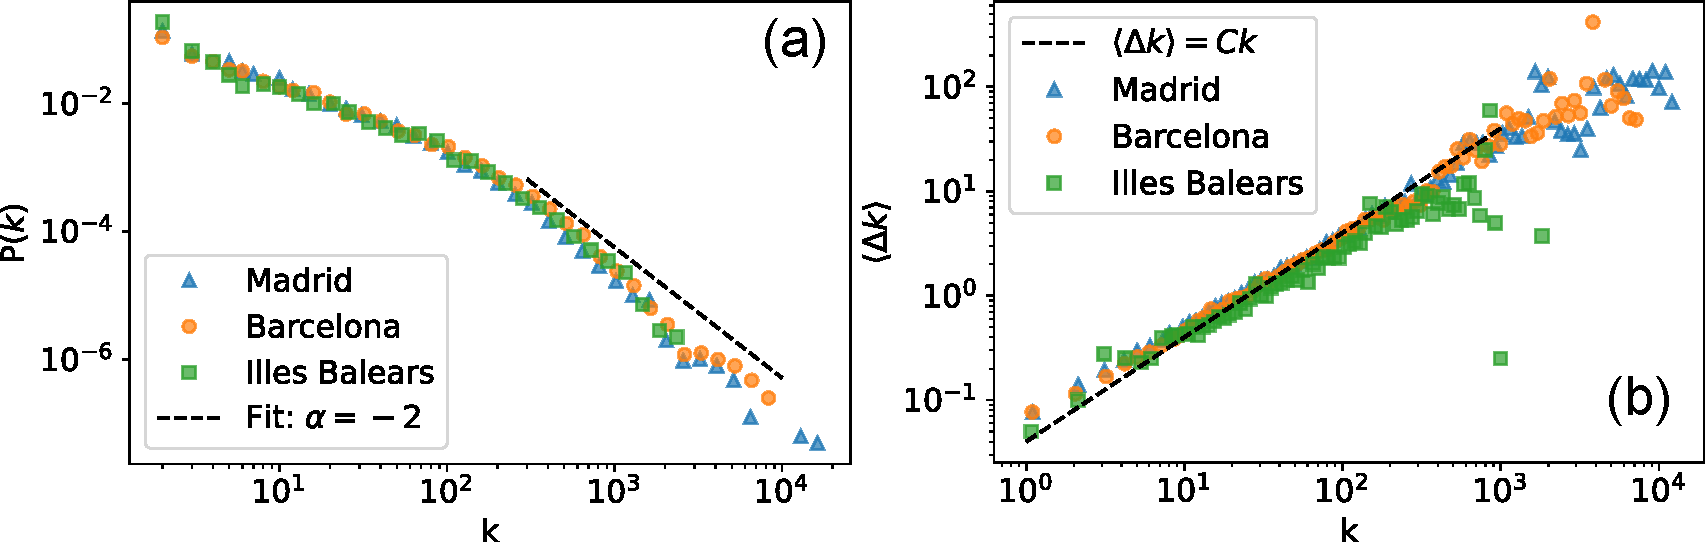
\includegraphics[width =\textwidth]{Figs/Idealista_dynamics/panel_degree.pdf}
	\caption[Preferential attachment to agencies.]{\label{fig:panel_degree}Preferential attachment to agencies. \textbf{(a)} Degree distribution of the agencies in the 3 regions. \textbf{(b)} Average degree increase of an agency as a function of the degree (listings posted) of the agency previously to the attachment. For both plots, different colors and markers indicate different regions or provinces. In \textbf{(a)}, the black dashed line shows a power-law distribution with exponent $\alpha  =-2$, and in \textbf{(b)} shows a linear increase with fitted slope $C = 0.04$.}
\end{figure}

In previous section, we have analyzed the listings' dynamics, just exploring how the total and active adds increase. However, the listings are not isolated entities, but they have a price, a location and are posted by a real estate agency. Now, we adress the decision-making process that house owners follow when they decide to sell/rent their properties through a real estate agency, and how it is correlated with the pricing and the location of the listings.

To this end, we build a temporal bipartite network between listings and agencies. At each time window, defined by an initial date $t_0$ and a final date $t_f$, we construct a bipartite network where listings are connected to the agency that posted it if the listing is active in any time $t'$, inside the temporal window $t_0 \leq t' \leq t_f$. Does not matter if the listing was removed after $t_f$ or if it was added before $t_0$, we consider all active listings in the time window. Note that this network is very simple, as a listing cannot be connected to more than one agency. As it is observed in the schematic representation of the temporal bipartite network in Fig. \ref{fig:temporal_bipartite}, as the window moves in time, the bipartite network changes structure, allowing us to infer the agency-listings dynamics.

\subsection{Preferential attachment}

Considering the cumulated network of all the listings posted during the whole period, we can analyze the degree distribution of the agencies. The degree of an agency in this context is the number of listings posted by the agency. As shown in Fig. \ref{fig:panel_degree}(a), the degree distribution of the agencies in the 3 regions follows a power-law distribution, highlighting the presence of very large agencies coexisting with several small agencies, in terms of the number of listings posted. This result suggests that agencies follow a preferential attachment mechanism, where the probability of a new listing being attached to an agency is proportional to the number of listings posted by the agency previously. This is a common mechanism in many real-world networks, such as the World Wide Web \cite{barabasi1999emergence}, citation networks \cite{redner1998popular}, transportation networks \cite{barrat2004architecture}. In the case of the housing market, this mechanism is a signature of the popularity of the agencies, as the more listings an agency has, the more likely it is to have new listings attached to it.

To verify if the underlying mechanism is indeed preferential attachment, we analyze the average degree increase of an agency as a function of the degree of the agency previously to the attachment. For this purpose, we build a bipartite network for a time window of 1 month and compute the increase of degree of the agencies after a week. This methodology allows us to track the real estate agencies one by one to see if there is indeed a degree increase biased by the degree of the agency previously to the attachment. We repeat this process for all the time windows in the period, and we average the results. As shown in Fig. \ref{fig:panel_degree}(b), the average degree increase of an agency is linearly correlated with the degree of the agency previously to the attachment. This result confirms that the agencies follow a preferential attachment mechanism, where the probability of a new listing being attached to an agency is directly proportional to the number of listings posted by the agency previously. However, this agency popularity in terms of degree is not the only key factor in the attachment process. The price of the listings and the location of the listings are also important factors that influence the decision-making process of the house owners.

\begin{figure}
    \centering
    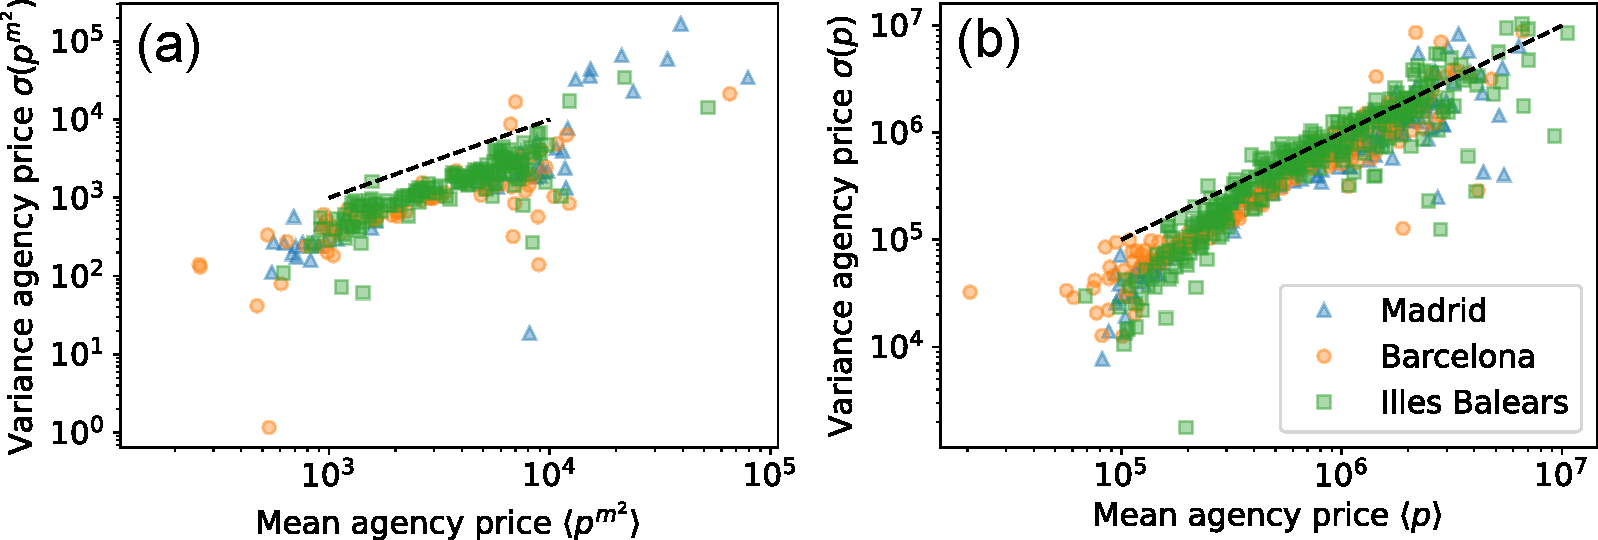
\includegraphics[width =\textwidth]{Figs/Idealista_dynamics/labeled_sigma_price.pdf}
	\caption[Variance of the agency price vs mean agency price.]{Variance of the listings price posted by an agency as a function of its mean price for the price per square meter \textbf{(a)} and the total price \textbf{(b)}. Different colors and markers indicate different regions or provinces. The black dashed line shows a linear fit with $\sigma(p) = \langle p \rangle$ for both plots. Here, $\langle \cdot \rangle$ stands for the average over the listings of an agency. \label{fig:sigma_price}}
\end{figure}

\subsection{Price correlations}

Since we have both the price and the surface area we compute the price per square meter of the listings, which is a common metric used in the real estate market. Both the price per square meter and the total price of the listings are distributed according to a log-normal distribution, an expected result in economic systems like ours \cite{ibragimov2015heavy}. The price range of an agency is defined by the mean price of its listings and its variance, which are found to be correlated (see Fig. \ref{fig:sigma_price}). For both, the price per square meter and the total price, the variance of the listings price posted by an agency is proportional to the mean price of the agency, such that the higher the listings prices of an agency, the higher the variance. This proportionality has been observed for population count in ecological contexts \cite{anderson1982variability, kilpatrick2003species}, and also recently in social systems \cite{chen2020scaling}, and it is known as Taylor's law \cite{taylor1961aggregation,eisler2008fluctuation}. In physics literature, this proportionality is known as fluctuation scaling \cite{eisler2008fluctuation}, and it is shown to be related with heavy tailed data \cite{brown2021taylor}, highlighting the heterogeneity in agencies pricing.

\begin{figure}
    \centering
    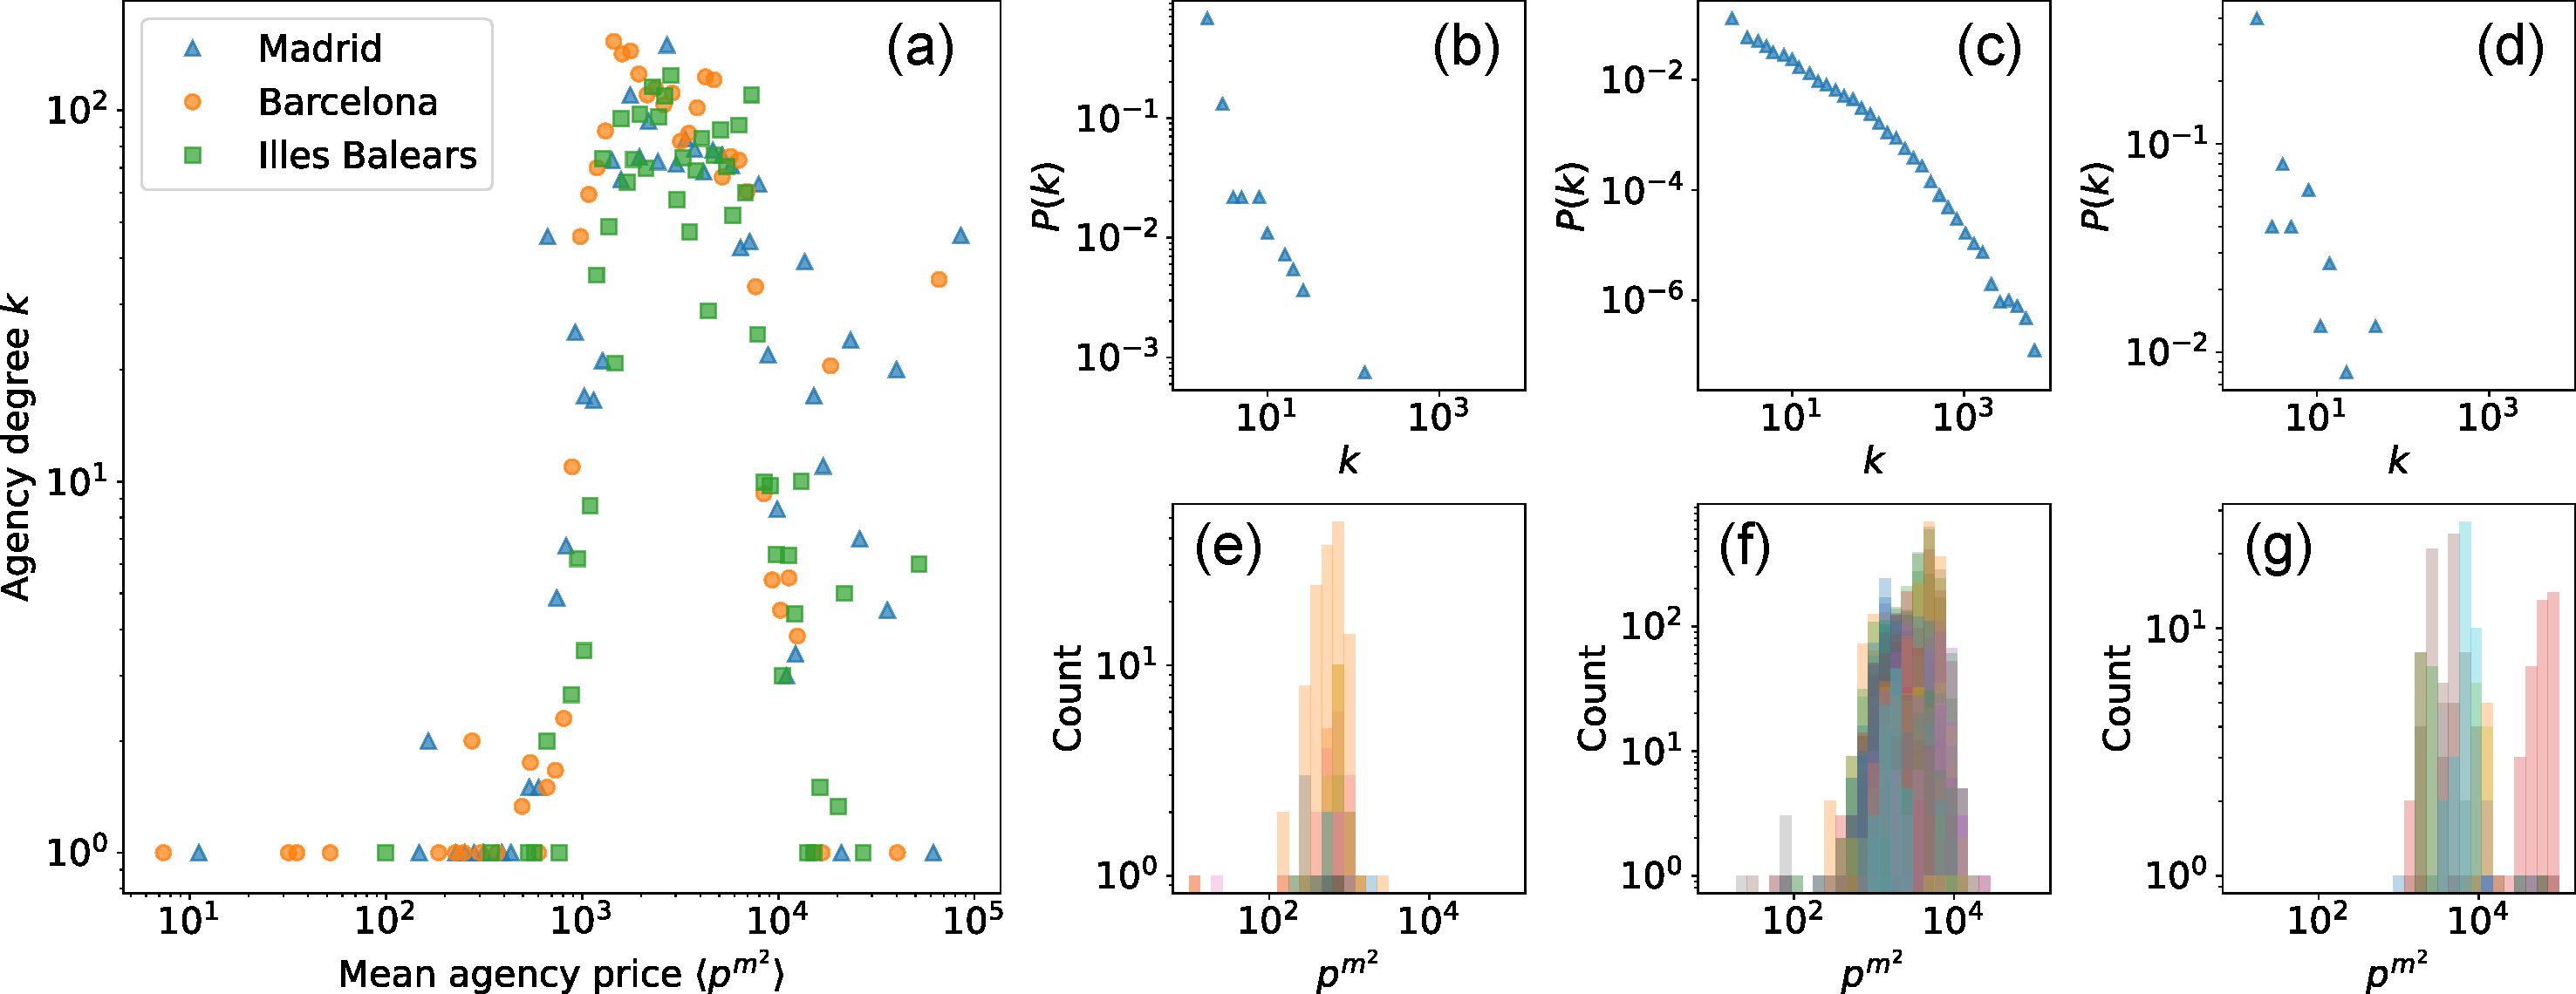
\includegraphics[width =\textwidth]{Figs/Idealista_dynamics/panel_price.pdf}
	\caption[Price segmentation by the degree.]{\textbf{(a)} Average degree (number of listings) of an agency as a function of its mean price per square meter. Different colors and markers indicate different regions or provinces. Degree distribution among the agencies \textbf{(b)-(c)-(d)} and price histograms for 60 representative agencies \textbf{(e)-(f)-(g)} at the different price segments: \textbf{(b)-(e)} $p^{{m}^2} < 800 \, \textup{\euro} / m^2$, \textbf{(c)-(f)} $800 \, \textup{\euro}  / m^2 < p^{{m}^2} < 10^4 \, \textup{\euro}  / m^2$, and \textbf{(d)-(g)} $p^{{m}^2} > 10^4 \, \textup{\euro}  / m^2$. These plots correspond to the Madrid housing market. For the price distributions, the colors indicate histograms for different agencies. $\langle \cdot \rangle$ stands for the average over the listings of an agency. \label{fig:panel_price}}
\end{figure}

Besides price itself, we analyze how correlated is the price of the listings of an agency with its degree in the bipartite network. As shown in Fig. \ref{fig:panel_price}(a), the average degree of an agency shows a non trivial dependence with the price per square meter. For low mean price, the degree values are very low. If we increase the price, we reach the typical prices in the market and degree increases very fast to a certain high value that keeps constant during a range of prices, but for very high prices, it decays again. This result suggests that agencies with low and high prices have few listings. The agencies with the highest number of listings are those with intermediate prices. This degree dependence allows us to segment the system in different price ranges according to how large is the mean degree. At the low prices segment (Fig. \ref{fig:panel_price}(b)-(e)), the degree distribution does not show a long tail anymore, and the agencies show a price distribution peaked at a certain price and with low fluctuations. For intermediate prices (Fig. \ref{fig:panel_price}(c)-(f)), the degree distribution exhibits the power-law behavior observed in Fig. \ref{fig:panel_degree}(a). In this price segment, the agencies show price distributions similar to a log-normal distribution, with a peak at a certain price and fluctuations around it. For high prices (Fig. \ref{fig:panel_price}(d)-(g)), the degree distribution is rather homogeneous (do not have a fat tail) and the price distribution of the agencies shows higher variance, since the agencies include both high prices and middle prices listings. This segmentation is an effect of the coexistence of generalist agencies, that post agencies in a wide range of prices, and specialist agencies, which focus on a specific submarket segment. Note that these results are consistent with the fluctuation scaling observed in Fig. \ref{fig:sigma_price}. 

So far, the price correlations described have been analyzed from a static point of view. Regarding price dynamics, we explore how the attachment of new listings is correlated with the price per square meter. As we did for the degree preferential attachment, we compute the mean agency price during a time window of 1 month and price of the new listings attached to the agency during the next week. This process is repeated for all the time windows in the period. When we average over possible values of the new listings price, we observe a positive correlation, similar to linear, between the mean agency price and the new listings attached price (see Fig. \ref{fig:attach_price}(a)). This correlation seems to be robust across the different regions, highlighting how listings with a certain price attach to agencies that work in a similar price range.

\begin{figure}
    \centering
    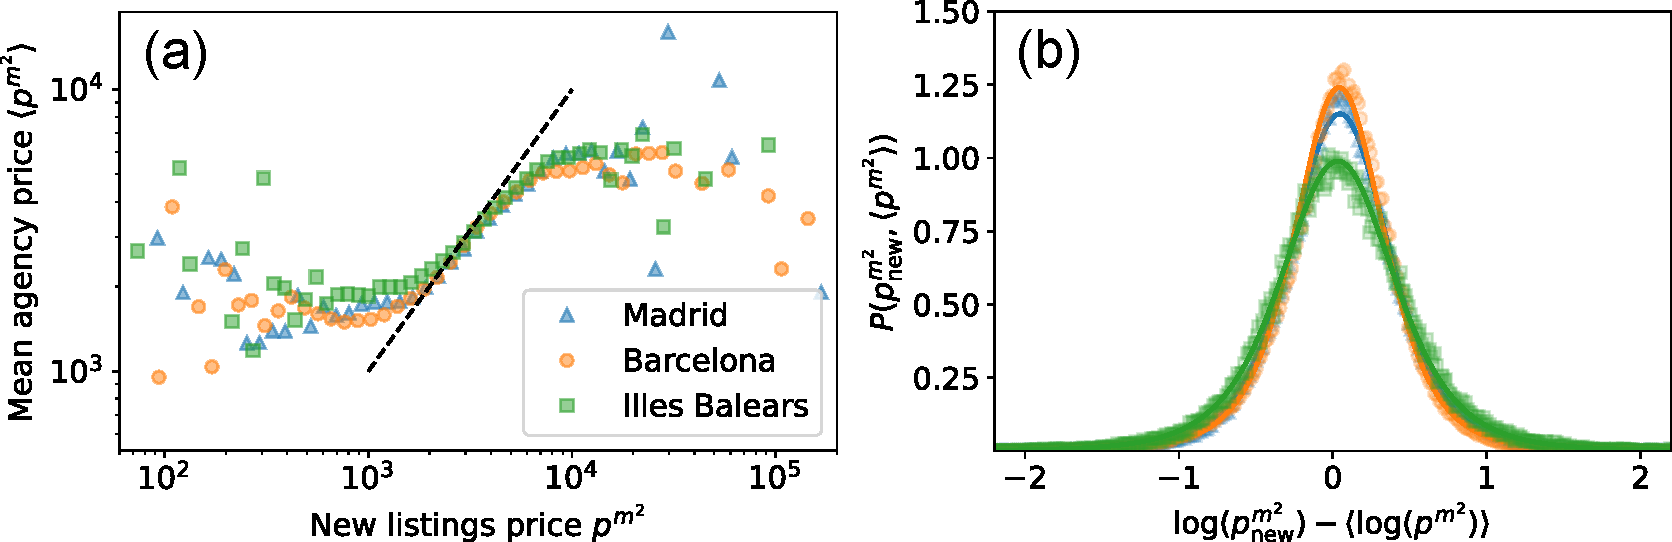
\includegraphics[width =\textwidth]{Figs/Idealista_dynamics/panel_attach_price.pdf}
	\caption[Attachment dynamics of new listings by price.]{Attachment of new listings by price. \textbf{(a)} Mean agency price per square meter as a function of the price of the new listing attached to the agency. Different colors and markers indicate different regions or provinces. The black dashed line shows a linear increase $\langle p^{{m}^2} \rangle = p^{{m}^2}_{\rm new}$. \textbf{(b)} Distribution of the logarithmic difference between the price of the new listing and the mean price of the agency. Different colors indicate different regions or provinces. $\langle \cdot \rangle$ stands for the average over the listings of an agency. Each solid colored line corresponds to a T-student fit for each region. The parameters are: $\nu = 5.47$, $\mu = 0.04$, $\sigma = 0.33$ for Madrid, $\nu = 4.62$, $\mu = 0.04$, $\sigma = 0.30$ for Barcelona, and $\nu = 4.49$, $\mu = 0.03$, $\sigma = 0.38$ for the Balearic Islands. $\nu$ is the degrees of freedom, $\mu$ is the location parameter, and $\sigma$ is the scale parameter. \label{fig:attach_price}}
\end{figure}

For each new attachment, we can compute how the price of a new listing attached fluctuates around the mean price of the agency. Fig. \ref{fig:attach_price}(b) shows the distribution of the logarithmic difference between the price of the new listing and the mean price of the agency. This distribution is found to be centered around $\log( p^{{m}^2}_{\rm new}) - \langle \log ( p^{{m}^2} ) \rangle \approx 0$, as expected from the previous result, and is well-fitted by a T-student distribution. Therefore, besides the preferential attachment, the listing price proportionality is an important factor of the housing market dynamics. When a new house is sold, is more likely to be sold by an agency with both, a high number of  active listings (degree) and a similar price range.

\subsection{Specialization in space}

It is said that in the real estate market, the three most important factors are location, location, and location \cite{rosen1974hedonic}. In this section, we focus on the spatial correlations of the listings. The location of the listings is well-defined by its coordinates, but the location of an agency is not so clearly defined. We define as the agency location in a time window, the center of mass (CM) of the active listings posted by the agency in that time window. This definition is a simplification that allows us to quantify the spatial correlations of the listings via the distance from the listings and the agency center of mass. Fig. \ref{fig:distance_panel}(a) shows the distribution of the distance between listings and the agency center of mass for the 3 regions. This distribution is computed for all the listings in the period, is peaked around $10^2$ m, and follows an exponential decay. In fact, for Barcelona and Madrid, the largest distance is around $10^5$ m, but for the Balearic Islands, we observe a longer tail that reaches $2.5 \times 10^5$ m. This occurs due to the natural spatial segmentation of the Balearic Islands and the presence of generalist agencies that post listings in different islands.

\begin{figure}
    \centering
    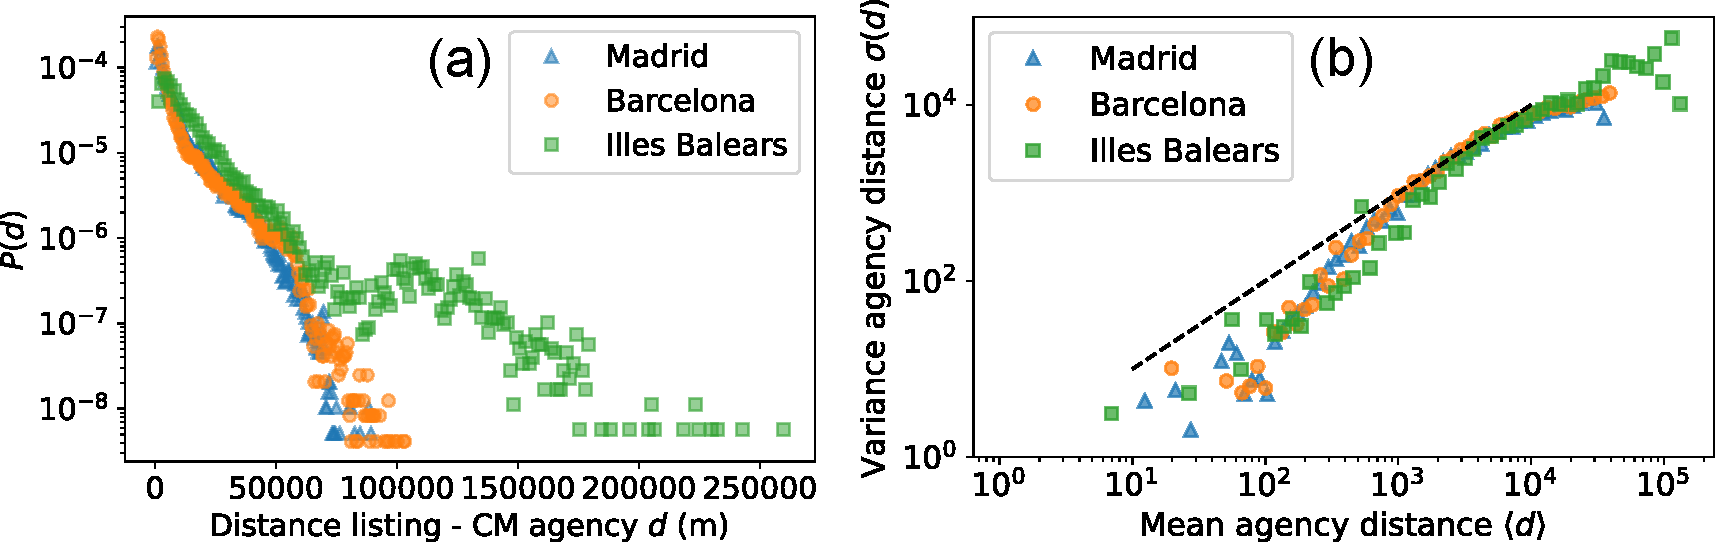
\includegraphics[width =\textwidth]{Figs/Idealista_dynamics/distance_panel.pdf}
	\caption[Distance correlations.]{\textbf{(a)} Distribution of the distance between listings of a certain agency and the center of mass of that same agency (mean location of the listings). \textbf{(b)} Variance of the listings distance to the agency center of mass of an agency as a function of its mean distance. The black dashed line shows a linear increase $\sigma(d) = \langle d \rangle$. Different colors indicate different regions or provinces. \label{fig:distance_panel}}
\end{figure}

As it occurred for the price of listings, the variance of the distance between the agency CM and the listings of an agency is proportional to the mean distance of the agency. This proportionality is shown in Fig. \ref{fig:distance_panel}(b) for the 3 regions studied, even though the relation is not as linear as for the price, specially for low mean agency distances. This result suggests that agencies with a higher effective radius $R$, defined as the mean distance $R = \langle d \rangle$, have a higher heterogeneity in the listings' location. Moreover, this fluctuation scaling process highlights the absence of a typical size of an agency in terms of  effective radius, going from large agencies that operate effectively everywhere, to localized agencies that focus on a specific region or neighborhood.

\begin{figure}
    \centering
    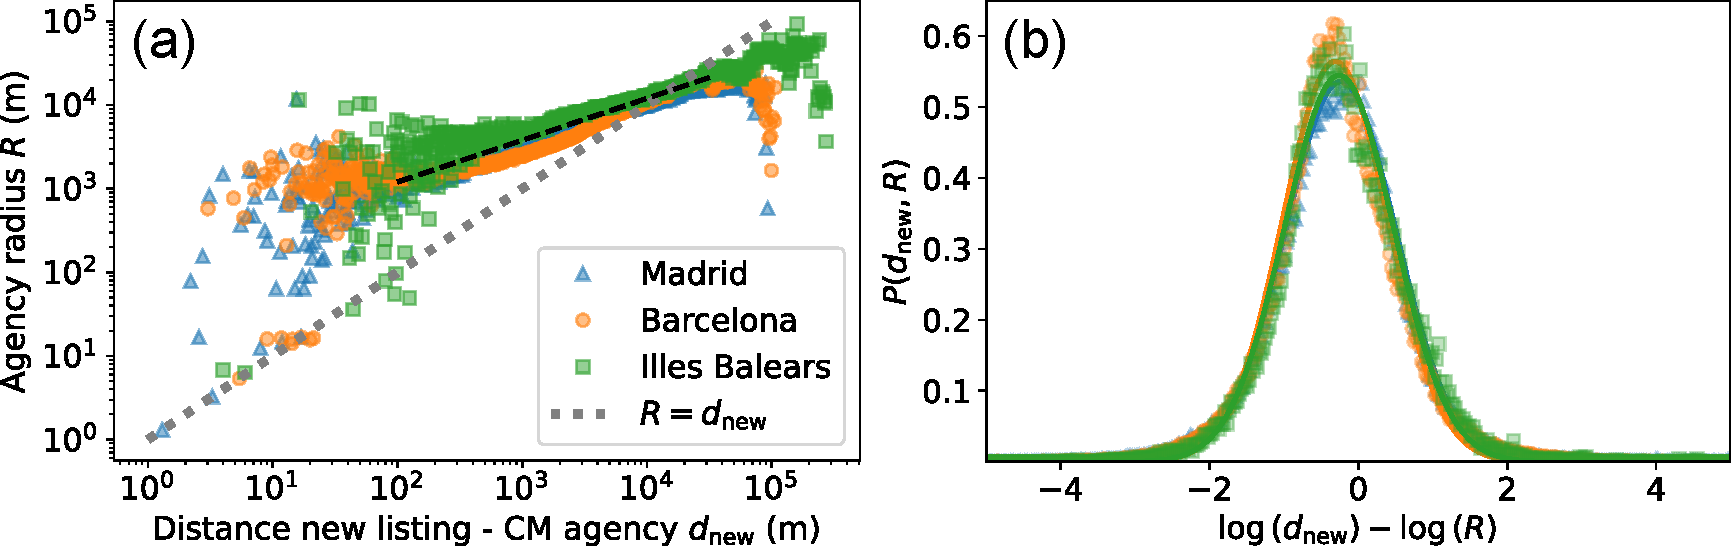
\includegraphics[width =\textwidth]{Figs/Idealista_dynamics/distance_attach.pdf}
	\caption[Attachment dynamics of new listings by distance.]{ Attachment dynamics of new listings by distance. \textbf{(a)} Agency effective radius (mean distance of the listings to the agency center of mass) as a function of the distance of the new listing (to the center of mass) attached to the agency. The black dotted grey line shows a linear increase $R = d_{\rm new}$, while the dashed black line shows a square root dependence $R = C \, d_{\rm new}^{1/2}$ being $C = 120$. \textbf{(b)} Distribution of the logarithmic difference between the distance of the new listing $d_{\rm new}$ and the effective radius of the agency $R$ (before the attachment). Different colors indicate different regions or provinces. Each solid colored line corresponds to a T-student fit for each region.  The parameters are: $\nu = 5.63$, $\mu = -0.25$, $\sigma = 0.69$ for Madrid, $\nu = 5.49$, $\mu = -0.30$, $\sigma = 0.67$ for Barcelona, and $\nu = 6.00$, $\mu = -0.25$, $\sigma = 0.67$ for the Balearic Islands. $\nu$ is the degrees of freedom, $\mu$ is the location parameter, and $\sigma$ is the scale parameter. \label{fig:distance_attach}}
\end{figure}

Regarding the dynamics, the location of a new listing also affects the attachment process to an agency. Fig. \ref{fig:distance_attach}(a) shows the effective radius as a function of the distance of the new listing attached to the agency. In this case, the scenario is very different to the price attachment. Here, the effective agency radius follows a proportional dependence to the distance listing - CM of the agency, but clearly sublinear (similar to $R \sim d_{\rm new}^{1/2})$. Thus, the majority of listings are attached to agencies with an effective radius larger or equal than the distance between the listing and the agency CM. This result is similar in all regions studied and consistent with the specialization of agencies in a certain area.

Moreover, as we did for the pricing and degree with a monthly window, we compute the distribution of the logarithmic difference between the distance of the new listing and the mean distance of the agency. Now, this distribution is not centered at $\log(d_{\rm new}) - \log(R) = 0$, but at negative values, as shown in Fig. \ref{fig:distance_attach}(b). Therefore, the new listings are attached to agencies where the effective radius is equal or larger than the distance listing - CM but with present exceptions to this process. Notice that this distribution comes from an analysis of a dynamical process, and the agency CM and effective radius are changing in time and so the attachment process. From this results, we can conclude that when a new house is sold, is more likely to be sold by an agency with a high number of listings, with a similar price range to the house hat also works in a similar area. These 3 mechanisms are the key factors that will compete and balance each other in the decision-making process of the house owners.

\section{Conclusions}

In this chapter, we have analyzed the dynamics of the housing market, using a comprehensive dataset of listings posted on an online platform for 3 provinces in Spain. We have shown that the listings' dynamics are non-stationary, with a weekly pattern in the number of active listings and a linear increase in the total number of listings. The listings' life distribution shows a fat tail, indicating irregular bursty dynamics, but the inter-activations time distribution not as heterogeneous as in other human activities. This process can be understood as a delayed degradation process, where listings are added to the platform at a constant rate, and they are removed after a certain time, similar to the attachment to a previous state in aging models. 

We have also shown that agencies follow a preferential attachment mechanism, where the probability of a new listing being attached to an agency is proportional to the number of listings posted by the agency previously, highlighting the presence of agency popularity in this market. Moreover, we found for both prices and distances (between add and agency center of mass), that the variance of the listings is proportional to the mean price or distance of the agency, showing a fluctuation scaling behavior. The presence of this relation in both magnitudes is a signature of heterogeneity and an underlying universal mechanism driving metadata in systems like this one to exhibit this Taylor's law behavior. The price of the listings is also correlated with the degree of the agency, showing a non-trivial dependence that allows to segment the market. 

For both, the distance and the price of a new house to be added into the offer system are key factors in the decision-making process of the house owners. So, in the housing market dynamics, there are 3 mechanisms competing directly: the popularity of the agency (preferential attachment), the price range of the listings of that agency (price proportionality), and the spatial specialization (distance lower than the agency radius). The balance of the importance on each of the mechanisms is what drives the housing market dynamics, and the results presented in this chapter serve as a basis to understand quantitatively emergent processes such as spatial specialization or price segmentation of the agencies.

The results presented in this chapter are based on a single dataset, and further work is needed to explore the generality of these results in other regions or countries. Nevertheless, it is important to remark that the results presented in this chapter were resilient to the different regions studied (Balearic Islands, Barcelona and Madrid), highlighting the robustness of the mechanisms found. Further work addressing the universality of these mechanisms need to be explored, as well as the exploration of other features, such as the price or distance correlation with the life of the listings in a certain agency, the spatial competition between agencies or the resilience of these mechanisms.

Further work could use this result to develop a model of the housing market dynamics, based on the idea similar to ``aging'' (explored in the first part of this thesis). This allows us to explore how the listings are posted on the online platform and how the agencies influence the decision-making process of the house owners. These models could be used to predict the future evolution of the housing market, which has important economic impact, as it can help to develop strategies to improve the housing market efficiency. Additionally, the understanding of the housing market dynamics could be useful for policymaking to predict market trends, and to develop strategies to reduce the housing market inequalities.